\chapter{Описание реализованного подхода}
\label{chapter2}

В данной главе описывается разработанный метод автоматизированного покрытия кода тестами на основе эволюционных алгоритмов.

\section{Постановка задачи}
Целью данной работы является создание платформы для автоматизированного покрытия программ тестами, учитывающими внутреннюю структуру тестируемой программы, на 
основе эволюционных алгоритмов и проверка разработанного метода на ряде модельных задач. Требования к данной работе:
\begin{itemize}
 \item Разработать метод автоматизированного покрытия тестами кода программ, работающих на \textit{JVM}.
 \item Провести сравнение разработанного метода с методом генерации случайных тестов на ряде модельных задач.
 \item Апробировать предложенный подход для покрытия тестами решения олимпиадной задачи Huzita~Axiom~6. 
\end{itemize}

\section{Общая схема решения}


На рисунке~\ref{pipeline} показана общая схема решения. При загрузке \textit{class}-файла тестируемой программы происходит модификация кода с целью получения 
траектории выполнения, а также считывания значений, переданных инструкциям ветвления, в процессе выполнения модифицированной программы. Заметим, что модификация 
кода тестируемой программы происходит таким образом, чтобы не изменился результат ее работы.

\begin{figure}[h!]
  \center{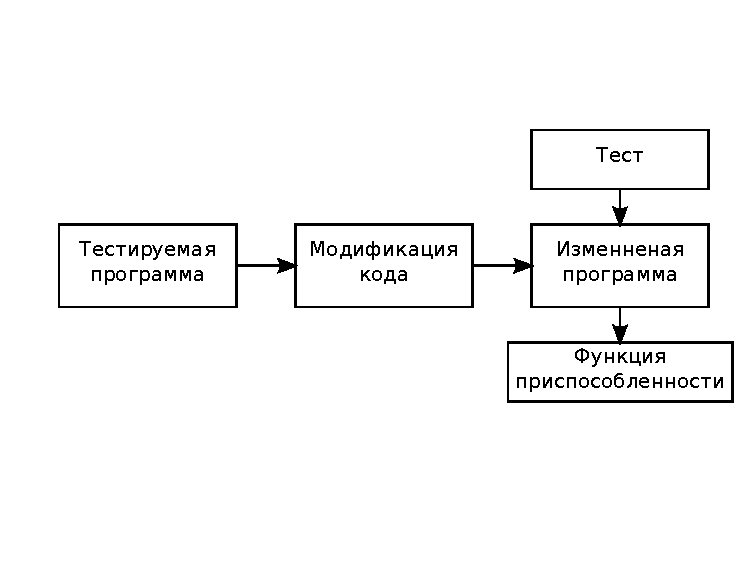
\includegraphics[width=0.6\textwidth]{pipeline.pdf}}
  \caption{Общая схема алгоритма}
  \label{pipeline}
\end{figure} 

После загрузки модифицированного кода происходит инициализация списка ветвлений, покрываемых инструкций. Будем называть целью заданное ветвление выбранной 
инструкции. Дальнейшее решение сводится к поиску набора тестов, обеспечивающих покрытие каждой цели.

Построение теста, покрывающего заданную цель, рассматривается как задачу оптимизации, решаемая с помощью эволюционных алгоритмов (ЭА). В качестве особи 
ЭА кодируется тест. С учетом требований к искомому тесту для особи определяются необходимые эволюционные операции: мутация и кроссовер. 

Для покрытия каждой цели используется свой экземпляр ЭА. Экземпляры ЭА создаются лишь для непокрытых целей. Если в процессе работы находится тест, 
покрывающий ранее непокрытую цель, то такой тест сохраняется.

После получения набора тестов, покрывающего выбранные цели, производится его минимизация с целью уменьшения накладных расходов при дальнейшем тестировании.

Таким образом, для запуска алгоритма необходимо:
\begin{itemize}
 \item задать список целей;
 \item сконфигурировать ЭА;
 \item обеспечить возможность многочисленных расчетов функции приспособленности.
\end{itemize}

\section{Функция приспособленности}
\label{sec:fitness_fun}
Функция приспособленности (ФП) дает количественную оценку того, насколько заданный тест покрывает выбранную цель. В данной работе ФП выбирается так, чтобы 
оценивать, насколько близка траектория выполнения программы к заданной цели.

\subsection{Функция расстояния до ветви}
\label{sec:branch_distance}
У некоторых инструкций ветвления лишь определенные ветви способствуют покрытию тестами выбранной цели, поскольку только они приводят к выполнению нужного 
фрагмента кода. Функция расстояния до ветви определяется таким образом, что ее минимальное значение достигается при прохождении по желаемому ветвлению.

Рассмотрим построение функции расстояния до нужной ветви на примере метода, код которого приведен на листинге~\ref{lst:branch_distance}.

\begin{snippet}[caption=Пример функции расстояния до ветви, label={lst:branch_distance}]
  def testMethod(x : Int) {
    if (10 <= x && x <= 15) {
      A()	// %*целевое ветвление*)
    }
    B()
  }
\end{snippet}

На рисунке~\ref{branch_distance} представлена блок-схема тестируемого метода. Заметим, что условие $10 \le x \le 15$ заменяется двумя инструкциями ветвления на 
этапе компиляции. В качестве функции расстояния до ветви в данном случае подойдут $10 - x$ и $x - 15$ для первой и второй инструкции ветвления соответственно. 

\begin{figure}[h!]
  \center{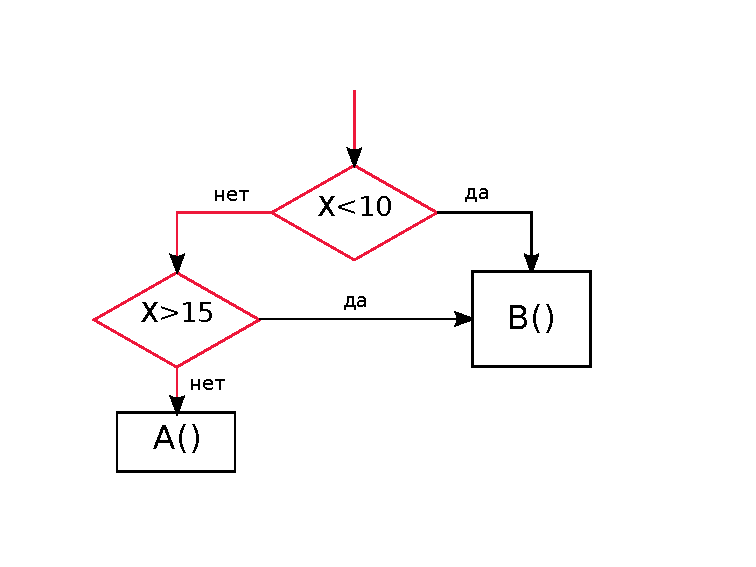
\includegraphics[width=0.5\textwidth]{branch_distance.pdf}}
  \caption{Блок-схема для листинга~\ref{lst:branch_distance}. Малиновым цветом выделена целевая траектория выполнения.}
  \label{branch_distance}
\end{figure}

Качество теста оценивается в зависимости от выбора функции расстояния до ветви. Так, например, сравнение значений типов long, double и float происходит при 
помощи специализированных инструкций, как \texttt{lcmp},  \texttt{dcmpg}, \texttt{dcmpl}, \texttt{fcmpg}, \texttt{fcmpl}. Результатом выполнения этих 
инструкций будет ноль, единица или минус единица и ветвление потока управления происходит с использованием соответствующих инструкций сравнения с нулем. Если в 
качестве значения функции расстояния до ветви использовать значения, переданные в инструкции ветвления напрямую, то эволюционный алгоритм будет работать плохо. 
Вместо них лучше использовать значения, переданные непосредственно в специализированные инструкции сравнения. Поэтому при подсчете функции расстояния до ветви 
необходимо анализировать код тестируемой программы.

\subsection{Следование опорной траектории}
\label{sec:track_based_fitness}
В данном случае предполагается, что траектория выполнения тестируемой программы должна совпадать с выбранной опорной траекторией. Опорная траектория либо 
задается человеком, либо генерируется автоматически на основе графа потока управления.

Рассмотрим опорную траекторию, состоящую из целей $C_1,C_2,..,C_k$. Пусть на некотором тесте была получена траектория $C_1,C_2,..,C_t,J,..$, где $J \neq 
C_{t+1}$. ФП представляется в виде пары двух чисел. Первое~--- длина общего префикса двух траекторий, а именно \texttt{t}. В качестве второго числа берется 
значение функции расстояния до ветви для цели $C_t$, поскольку именно в ней разошлись две траектории. При сравнении двух особей более приспособленной считается 
та, у которой первое число ФП больше. Если первые числа ФП равны, то лучше та особь, у которой второе число меньше.

Рассмотрим пример на рис.~\ref{singlepathfitness}. Опорная траектория выделена малиновым цветом. Зелеными кружками помечена траектория выполнения программы. 
Инструкция, отмеченная темно-зеленым кружком, соответствует $C_t$ и в ней происходит расхождение траекторий. Длина общего префикса отмеченных траекторий 
равна трем.

\begin{figure}[h!]
  \center{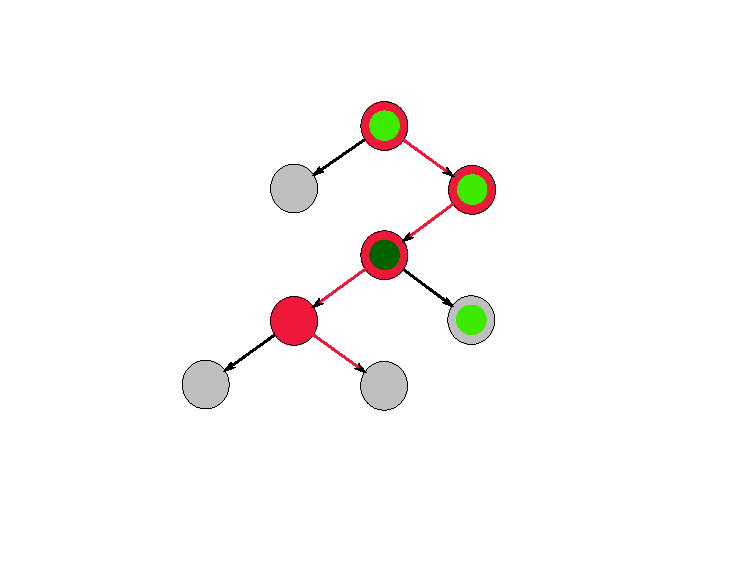
\includegraphics[width=0.5\textwidth]{singlepathfitness.pdf}}
  \caption{Пример расхождения с опорной траекторией}
  \label{singlepathfitness}
\end{figure}

Существуют другие варианты построения функции приспособленности на основе следования опорной траектории. Допустим, ни одна траектория выполнения программы не 
может следовать выбранной опорной траектории во всех инструкциях. В таком случае невозможно найти тест, покрывающий выбранную цель. Однако если в 
качестве первого числа функции приспособленности взять наибольший номер инструкции, общей для двух траекторий, то такой тест может быть сгенерирован.

Недостатком такого подхода является необходимость выбора опорной траектории, поскольку возможно большое число траекторий, проходящих по заданному ветвлению. 
При этом время работы алгоритма сильно зависит от выбора опорной траектории, так как не вдоль всех траекторий можно сгенерировать тест.

\subsection{Приближение по многим направлениям}
Обычно при покрытии выбранной цели нет предпочтений насчет траектории, вдоль которой надо покрывать. Таким образом, необходимо выбрать опорную траекторию, либо 
задать функцию приспособленности, рассматривающую приближение вдоль всех возможных траекторий.

Расстоянием \texttt{d(x, y)} между инструкцией \texttt{x} и инструкцией \texttt{y} будем считать минимальную длину пути от инструкции \texttt{x} до инструкции 
\texttt{y} в графе потока управления. Если такой путь не существует, то $d(x, y) = \infty$. В качестве расстояния \texttt{d(T, x)} от траектории $T={t_1, 
t_2,...,t_k}$ до инструкции \texttt{x} возьмем $\min\limits_{i=1..k}{d(t_i, x)}$.


Пусть выбрана цель \texttt{c} и заданному тесту \texttt{t} соответствует траектория выполнения \texttt{T}. Тогда в качестве значения функции приспособленности 
берется пара чисел, первое из которых равно \texttt{d(T, c)}, а второе~--- минимальному значению функции расстояния до ветви для инструкции \texttt{i} на 
траектории \texttt{T}, такой что $d(i,c) = d(T,c)$. 

Рассмотрим пример на рис.~\ref{multipathfitness}. На нем изображены две различные траектории выполнения одного и того же фрагмента кода, выделенные зеленым 
цветом. Цель \texttt{c} выделена малиновым цветом. Темно-зеленым цветом выделена инструкция \texttt{i}. Обе траектории находятся на расстоянии до цели, равном 
одному условному переходу.

\begin{figure}[h!]
  \center{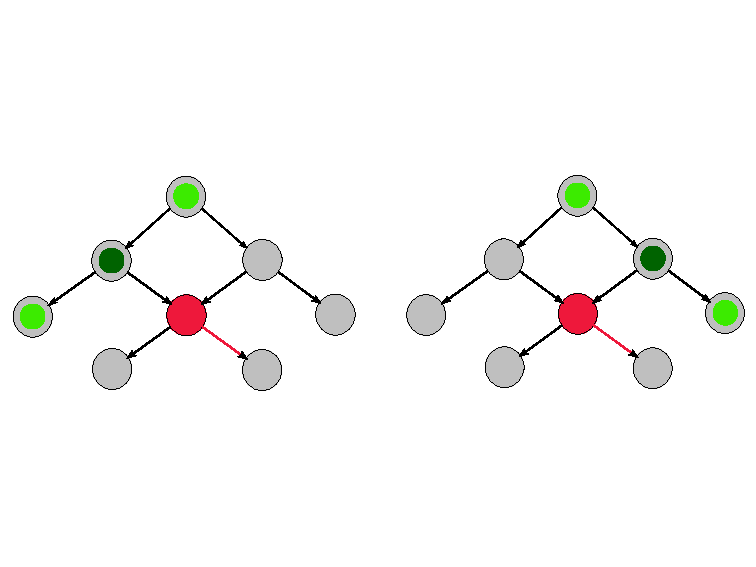
\includegraphics[width=0.8\textwidth]{multipathfitness.pdf}}
  \caption{Пример приближения по многим направлениям}
  \label{multipathfitness}
\end{figure}

В данном примере, при совпадении второго числа в функции приспособленности, количественные оценки для обеих траекторий будут одинаковые, но качественно эти 
траектории различаются. Таким образом, при данном определении функции приспособленности одинаковые количественные оценки могут соответствовать качественно 
различным тестам.          

\section{Модификация кода}

Модификации кода тестируемой программы не должны изменять результат ее работы. Для работы с \textit{class}-файлами используется библиотека 
ASM~4.0~\cite{asm_lib}, предоставляющая доступ к списку инструкций. Базовый интерфейс применяемых модификаций приведен на листинге~\ref{lst:modification}.

\begin{snippet}[caption=Типаж модификации кода тестируемой программы, label={lst:modification}]
  import org.objectweb.asm.tree.{ClassNode, MethodNode}

  trait CodeModification {
    protected def onMethod(cn : ClassNode, mn: MethodNode)
  
    def onClass(cn : ClassNode) {
      cn.methods.iterator.foreach{ x =>
	onMethod(cn, x.asInstanceOf[MethodNode])
      }
    }
  }
\end{snippet}

Для модификации кода метода необходимо переопределить метод \texttt{onMethod}, входными аргументами которого являются ссылки на инструкции модифицируемого 
метода и класса, в котором этот метод определен. Для композиция двух модификаций метод \texttt{onMethod} определяется как последовательность вызовов методов 
\texttt{onMethod} этих модификаций. Класс композиции представлен на листинге~\ref{lst:composition}.

\begin{snippet}[caption=Композиция модификаций кода тестируемой программы, label={lst:composition}]
  import org.objectweb.asm.tree.{ClassNode, MethodNode}

  class Composition(a : CodeModification, b : CodeModification) extends CodeModification {
    protected def onMethod(cn : ClassNode, mn: MethodNode) {
      a.onMethod(cn, mn)
      b.onMethod(cn, mn)
    }
  }
\end{snippet}

Работа с кодом программы разделена на два этапа: на первом формируется внутреннее представление программы в виде графа потока управления, на втором~--- 
код модифицируется с целью считывания траектории выполнения программы и другой информации о процессе выполнения.

\subsection{Граф потока управления}
Библиотека \texttt{ASM} предоставляет доступ к списку инструкций каждого метода. Однако для структурного тестирования необходимо построение графа потока 
управления. 

\begin{definition}
Графом потока управления программы \texttt{F} называется ориентированный граф $G=(N, E, s, F)$, где \texttt{N}~--- множество вершин, \texttt{E}~--- множество 
ребер, \texttt{s}~--- входная инструкция, \texttt{F}~--- множество вершин, завершающих выполнение программы.
\end{definition}

Каждой вершине $n \in N$ графа потока управления соответствует инструкция \textit{JVM}. Ребром $e = (n_i, n_j)$ же является переход от инструкции $n_i$ к 
инструкции $n_j$.

Для построения графа потока управления используется типаж анализатора кода, представленный на листинге~\ref{lst:asm_analyzer}. При помощи дополнительных 
типажей анализатор индексирует инструкции ветвления, а также сохраняет построенный граф потока управления.

\begin{snippet}[caption=Типаж анализатора кода, label={lst:asm_analyzer}]
  import org.objectweb.asm.tree.{ClassNode, MethodNode}
  
  trait AsmControlFlowAnalyzer extends CodeModification { 
    needs : InstructionRegister with MethodRegister =>

    protected override def onMethod(cn : ClassNode, mn: MethodNode) {
      ...
    }
  }
\end{snippet}

\subsection{Считывание траектории выполнения программы}
Для анализа выполнения программы на заданном тесте считывается траектория выполнения, а именно последовательность инструкций ветвления и значения переданные им 
во время выполнения. Для идентификации инструкций ветвления используется нумерация, введенная при построении графа потока управления. 

Для считывания значений во время выполнения программы определен ряд методов, каждый из которых соответствует определенному типу инструкции ветвления. При работе 
с несколькими потоками последовательность инструкций ветвления будет составлена для каждого потока в отдельности~\cite{threadlocal}.

Рассмотрим модификацию кода программы, необходимую для считывания траектории выполнения. Для каждого профилируемого метода вводятся дополнительные локальные 
переменные. Перед выполнением инструкции ветвления выполняются следующие действия:
\begin{enumerate}
 \item Значения со стека операндов сохраняются в дополнительные локальные переменные.
 \item Состояние стека операндов восстанавливается из локальных переменных.
 \item Вызывается метод для считывания значений во время выполнения.
 \item Восстанавливается состояние стека операндов для дальнейшей работы программы.
\end{enumerate}

\section{Минимизация набора тестов}

Минимизация набора тестов является частным случаем задачи о минимальном покрытии множества. Пусть имеется множество тестов $T$. Для каждого теста $t \in T$ 
известно множество фрагментов кода, которые он покрывает. Требуется построить минимальное по мощности множество $T_{opt} \subset T$, такое что: 
$\bigcup\limits_{t \in T_{opt}}Cov(t) = \bigcup\limits_{t \in T}Cov(t)$.

В работе \cite{minimization} показано, что данная задача является \textit{NP}-полной. По причине чрезмерных затрат вычислительных ресурсов 
требуется применять приближенные методы.

Рассмотрим жадный алгоритм, решающий данную задачу:
\begin{enumerate}
 \item Пусть множество $X$~--- множество выбранных тестов, $P = \bigcup\limits_{t \in T}Cov(t)$, а множество $Z$~--- множество покрытых им фрагментов кода. 
Изначально $X, Z = \emptyset$.
 \item Если $Z = P$, прекратить работу, решение задачи $T_{opt} = X$.
 \item Выбрать такое $t \in T$, что $Cov(t) \cap (P / Z)$ максимально.
 \item $X = X \cup {t}$, $Z = Z \cup Cov(t)$, перейти к шагу 2.
\end{enumerate}

Время работы простейшая реализация данного алгоритма имеет асимптотическую оценку $O(|T|^2 \cdot |P|)$.  В работе~\cite{minimization_characterization} 
показано, что данный алгоритм генерирует в худшем случае ответ, превосходящий оптимальный в $O(log|P|)$ раз. Однако на практике для многих входных данных он 
дает ответ, отличающийся от оптимального не более чем на 10\%.

\section{Выводы по главе \ref{chapter2}}
Формализована цель работы: создание платформы для автоматизированного покрытия программ тестами на основе эволюционных алгоритмов. Описан предлагаемый подход. 
Предложен способ задания функции приспособленности, рассматривающий приближение по многим направлениям.